% Copyright 2004 by Till Tantau <tantau@users.sourceforge.net>.
%
% In principle, this file can be redistributed and/or modified under
% the terms of the GNU Public License, version 2.
%
% However, this file is supposed to be a template to be modified
% for your own needs. For this reason, if you use this file as a
% template and not specifically distribute it as part of a another
% package/program, I grant the extra permission to freely copy and
% modify this file as you see fit and even to delete this copyright
% notice. 

\documentclass{beamer}

\usepackage{xcolor}
\usepackage{CJKutf8}
\usepackage{rotating}
\usepackage{subfigure}
\usepackage{graphicx}
\usepackage{algorithm}
\usepackage{algorithmicx}
\usepackage{amsmath}
\usepackage{amssymb}
\usepackage[noend]{algpseudocode}
\usepackage{wallpaper}
\usepackage{animate}
\usepackage[backend=bibtex,sorting=none,maxcitenames=5,maxbibnames=5,hyperref=true,block=none,firstinits=true]{biblatex}
\bibliography{oral}
\algdef{SE}[DOWHILE]{Do}{DoWhile}{\algorithmicdo}[1]{\algorithmicwhile\ #1}%
\renewcommand{\algorithmicrequire}{\textbf{Input:}}
\renewcommand{\algorithmicensure}{\textbf{Output:}}
\newcommand{\var}[1]{\text{\texttt{#1}}}
\newcommand{\func}[1]{\text{\textsl{#1}}}


% table
\usepackage[normalem]{ulem}
\useunder{\uline}{\ul}{}
\usepackage{multirow}
\usepackage{tabularx}

\algdef{SE}[DOWHILE]{Do}{DoWhile}{\algorithmicdo}[1]{\algorithmicwhile\ #1}%

\usetheme{Madrid} % origin
\setbeamercolor{structure}{fg=violet}

\author{ 
    Chi-Ming Lee
}

\institute[NTHU EE] % (optional, but mostly needed)
{
    Department of Electrial Engineering\\
    National Tsing Hua University
}

\date{\today}

\AtBeginSubsection[]
{
    \begin{frame}<beamer>{Outline}
        \tableofcontents[currentsection,currentsubsection]
    \end{frame}
}

\begin{document}
\setbeamertemplate{background canvas}{\CenterWallPaper{.30}{./assets/nthu_watermark.eps}}
\begin{CJK}{UTF8}{bkai}

    \title[DeAr DSP]{ DeAr: 適用於異質系統架構之高效率且彈性的數位訊號處理器設計}
    \subtitle{DeAr: An Efficient and Flexible Digital Signal Processor Design for Heterogeneous System Architecture}

    \begin{frame}
        \titlepage
    \end{frame}

    \begin{frame}{Outline}
        \tableofcontents
        % You might wish to add the option [pausesections]
    \end{frame}

    % Section and subsections will appear in the presentation overview
    % and table of contents.

    \section{Introduction}

    \subsection{Motivation}

    \begin{frame}{Motivation (1/2)}
        \begin{itemize}
            \item <2->{
                    Evolution of wireless standards drives the quest for a new Digital Signal Processor (DSP)
                }
            \item <3->{
                    E.g., LTE-A demands 10 times transmission rate than LTE
                    \begin{itemize}
                        \item {
                                Heavy arithmetic (throughput)
                            }
                        \item {
                                Fast evolving demodulation algorithms (flexibility)
                            }
                        \item {
                                Endurance still matters (power-efficiency)
                            }
                    \end{itemize}
                }
            \item <4->{ 
                    DSP datapath has gone beyond scalar for higher throughput
                    \begin{itemize}
                        \item Very Long Instruction Word (VLIW)
                        \item Application Specific Instruction-set Processor (ASIP)
                    \end{itemize}
                }
            \item <5->{
                    Unfortunately, VLIW and ASIP are opposite extreme cases...
                    \begin{itemize}
                        \item VLIW: good flexibility and bad power-efficiency
                        \item ASIP: good power-efficiency and bad flexibility
                    \end{itemize}
                }
        \end{itemize}
        \vspace{1em}
        \centering
        \only <6->{\large{\textbf{ACHIEVING BOTH FLEXIBILITY AND POWER-EFFICIENCY IS A CHALLENGE!}}}
    \end{frame}

    \begin{frame}{Motivation (2/2)}
        \begin{itemize}
            \item <2->{
                    Heterogeneous computing, a system with multiple types of processors, is gaining momentum
                    \begin{itemize}
                        \item {
                                CPU handles control-intensive tasks
                            }
                        \item {
                                DSP, GPU and FPGA handles data-intensive tasks for acceleration
                            }
                    \end{itemize}
                }
            \item <3->{
                    Industry standard for heterogeneous computing, \textit{Heterogeneous System Architecture}~\cite{systemspec} emerged in 2012.
                    \begin{itemize}
                        \item {
                                Proposed by leading semiconductor companies%, AMD, ARM, MediaTek, Samsung, Texas Instrument, etc, 
                            }
                        \item {
                                Has opened a new era for embedded computing %platforms.
                            }
                    \end{itemize}
                }
            \item <4->{
                    Designing a novel DSP which is also compatible with HSA...
                }
        \end{itemize}
        \vspace{1em}
        \centering
        \only <5->{\large{\textbf{A TIGER WITH WINGS!!}}}
    \end{frame}


    \subsection{Contribution}

    \begin{frame}{Contribution}
        \begin{itemize}
            \item <2->{
                    We present \textbf{Dual-thread Architecture} (\textbf{DeAr}) DSP, which achieves both power-efficiency and flexibility.
                    \begin{itemize}
                        \item {
                                Simultaneous Multi-threading 
                            }
                        \item {
                                Flexible forwarding bus
                            }
                        \item {
                                Multi-banked RF with implicit addressing
                            }
                    \end{itemize}
                }
            \item <3->{
                    A novel scheduling algorithm, HDFG-based scheduling is proposed
                    \begin{itemize}
                        \item Beyond data flow graph (DFG) analysis
                        \item Optimizing \textbf{power dissipation}, \textbf{flexibility} and \textbf{Operations per Cycle} (OPC)
                    \end{itemize}
                }
            \item <4->{
                    We also propose a framework to integrate DeAr with HSA
                    \begin{itemize}
                        \item {
                                Architecture framework
                            }
                        \item {
                                Compilation framework
                            }
                    \end{itemize}
                }
            \item <5->{
                    Compared with VLIW and ASIP respectively, DeAr saves: 
                    \begin{itemize}
                        \item {
                                \textbf{20.3\%--13.1\%} and \textbf{31.8\%--2.2\%} of power
                                }
                            \item {
                                    \textbf{36.1\%--31.5\%} and \textbf{28.2\%--5.7\%} of area
                                    }
                            \end{itemize}
                        }
                \end{itemize}
            \end{frame}

            \section{Background}
            \subsection{Common DSP Datapaths}
            \begin{frame}{Very Long Instruction Word (VLIW)}
                \begin{columns}
                    \begin{column}{0.4\textwidth}
                        \begin{figure}[!ht]
                            \centering
                            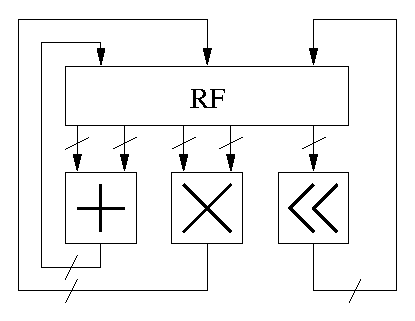
\includegraphics[width=0.9\textwidth]{./figs/vliw.eps}
                            \caption{VLIW datapath}
                        \end{figure}
                    \end{column}
                    \begin{column}{0.6\textwidth}
                        \begin{itemize}
                            \item <2-> {Each function unit (FU) works independently with dedicated ports in RF
                                }
                            \item <3-> {Pros:
                                    \begin{itemize}
                                        \item Multi-issue datapath \\ $\implies$ High operations per cycle (OPC)
                                        \item No dependency among FUs \\ $\implies$ Good flexibility
                                    \end{itemize}
                                }
                            \item <4-> {Cons:
                                    \begin{itemize}
                                        \item Worst-case port count in RF \\ $\implies$ Severe cost in power and area
                                        \item Write back for every operation \\ $\implies$ Increasing power cost
                                    \end{itemize}
                                }
                        \end{itemize} 
                    \end{column}
                \end{columns} 
            \end{frame}

            \begin{frame}{Application Specific Instruction Set Processor (ASIP)}
                \begin{columns}
                    \begin{column}{0.45\textwidth}
                        \begin{figure}[!ht]
                            \centering
                            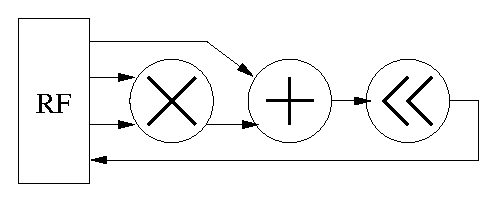
\includegraphics[width=0.9\linewidth]{./figs/cascade.eps}
                            \caption{ASIP datapath}
                        \end{figure}
                    \end{column}
                    \begin{column}{0.55\textwidth}
                        \begin{itemize}
                            \item <2-> {Composite-ALU ASIP proposed by Ou~\textit{et. al.}~\cite{cascade}}
                            \item <3-> {FUs are configured or cascaded in a special manner}
                            \item <4-> {Pros:
                                \begin{itemize}
                                    \item Composite operation support \\ $\implies$ high OPC
                                    \item Special-case port count in RF \\ $\implies$ Less cost in power and area
                                    \item Inherent FU forwarding path \\ $\implies$ Reducing power cost
                                \end{itemize}
                                }
                            \item <5-> {Cons:
                                \begin{itemize}
                                    \item Fitting particular applications only \\ $\implies$ Poor flexibility
                                \end{itemize}
                                }
                        \end{itemize} 
                    \end{column}
                \end{columns} 
            \end{frame}
            %\begin{frame}{Transport-triggered Architecture (TTA)}
            %    \begin{itemize}
            %        \item foo
            %        \item bar
            %    \end{itemize}
            %    \begin{figure}[!ht]
            %        \centering
            %        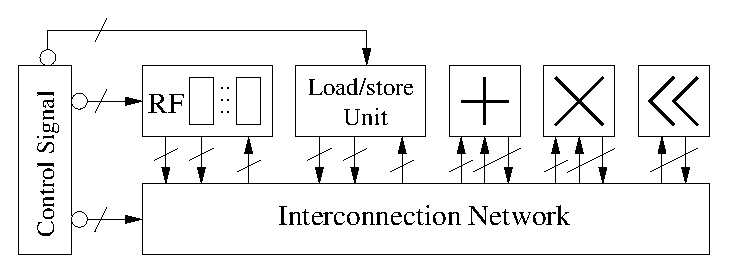
\includegraphics[width=0.6\linewidth]{./figs/tta.eps}
            %        \caption{TTA example}
            %    \end{figure}
            %\end{frame}

            \subsection{Heterogeneous System Architecture}
            \begin{frame}{Key Concepts of HSA}
                \begin{itemize}
                    \item <2->{Heterogeneous multi-core platform
                            \begin{itemize}
                                \item Particular processors (agents) handles particular tasks% --- better power efficiency
                            \end{itemize}
                        }
                    \item <3->{Heterogeneous System Architecture Intermediate Language (HSAIL)
                            \begin{itemize}
                                \item Providing an unified programming language %of heterogeneous cores
                                \item Single Program Multiple Data (SPMD) programming model
                            \end{itemize}
                        }
                    \item <4->{Shared Virtual Memory (SVM)
                            \begin{itemize}
                                \item Eliminating redundant transfer among agents
                                \item Passing pointers instead --- alleviating communication overhead
                            \end{itemize}
                        }
                    \item <5->{Architectural Queuing Language (AQL)
                            \begin{itemize}
                                \item Communication protocol for agents via AQL-queues
                                \item Task dispatching, information exchanging, synchronization, etc.
                            \end{itemize}
                        }
                \end{itemize} 
            \end{frame}

            \begin{frame}{HSA Platform Example}
                \begin{figure}[!ht]
                    \centering
                    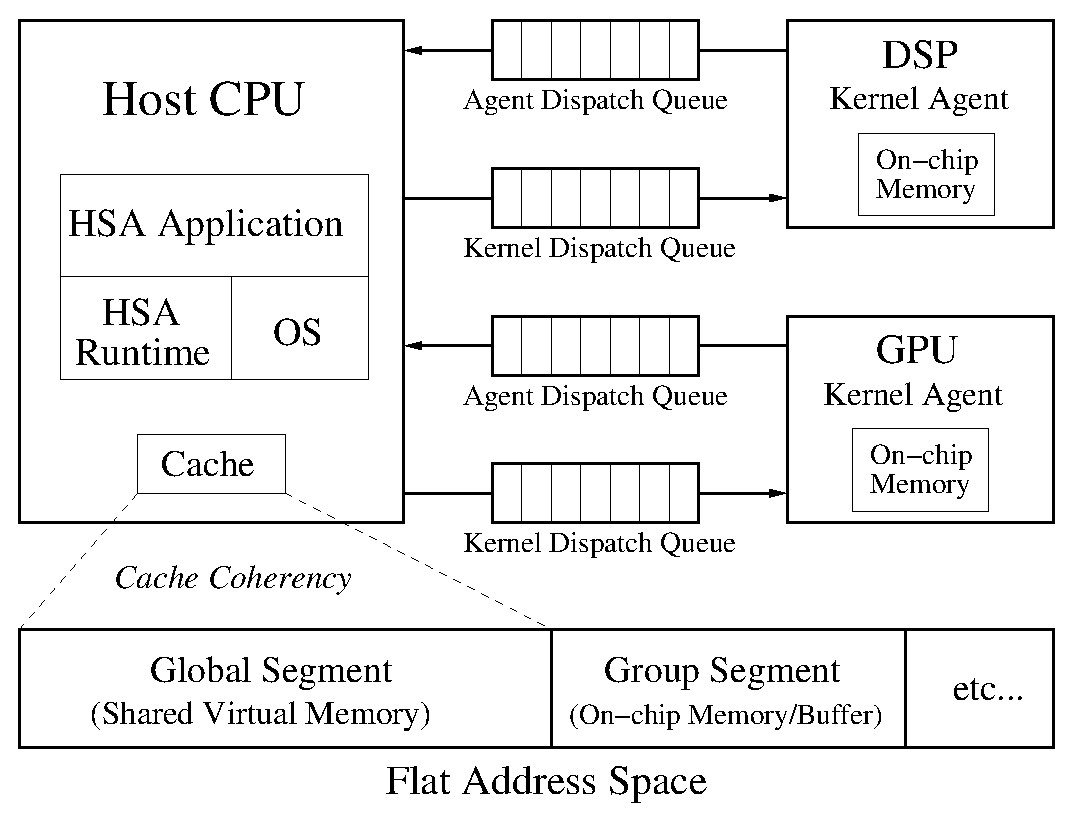
\includegraphics[width=0.8\textwidth]{./figs/systemspec.eps}
                    \label{fig:systemspec}
                \end{figure}
            \end{frame}

            \begin{frame}{Execution Hierarchy}
                \begin{figure}[t] 
                    \centering
                    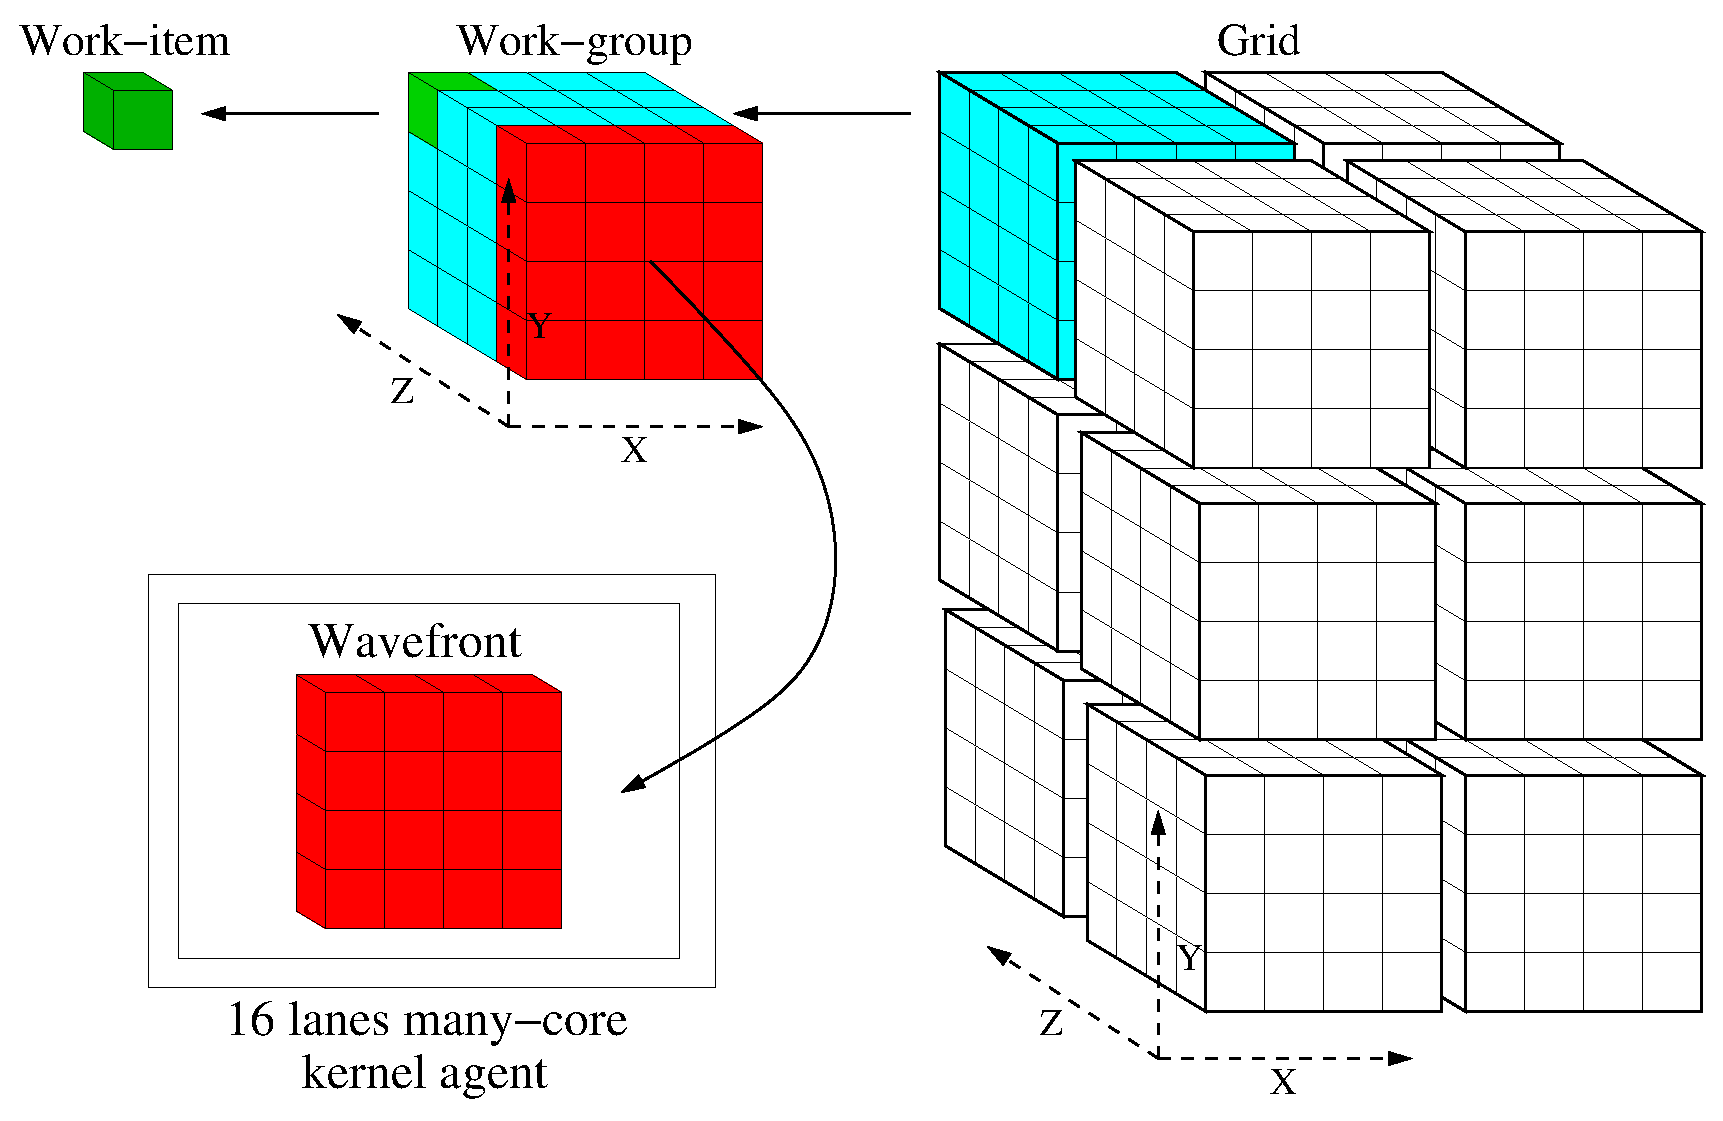
\includegraphics[width=0.7\textwidth]{./figs/grid.eps}
                    \label{fig:grid}
                \end{figure}%
                \begin{itemize}
                    \item <2-> {Work-item: primitive execution unit with dedicated registers}
                    \item <3-> {Work-group: a set of work-items sharing local memory}
                    \item <4-> {Grid: Assembly of all work-groups in the context}
                \end{itemize}
            \end{frame}

            %\begin{frame}{Software Infrastructure of HSA}
            %    \begin{figure}[!ht] 
            %        \centering
            %        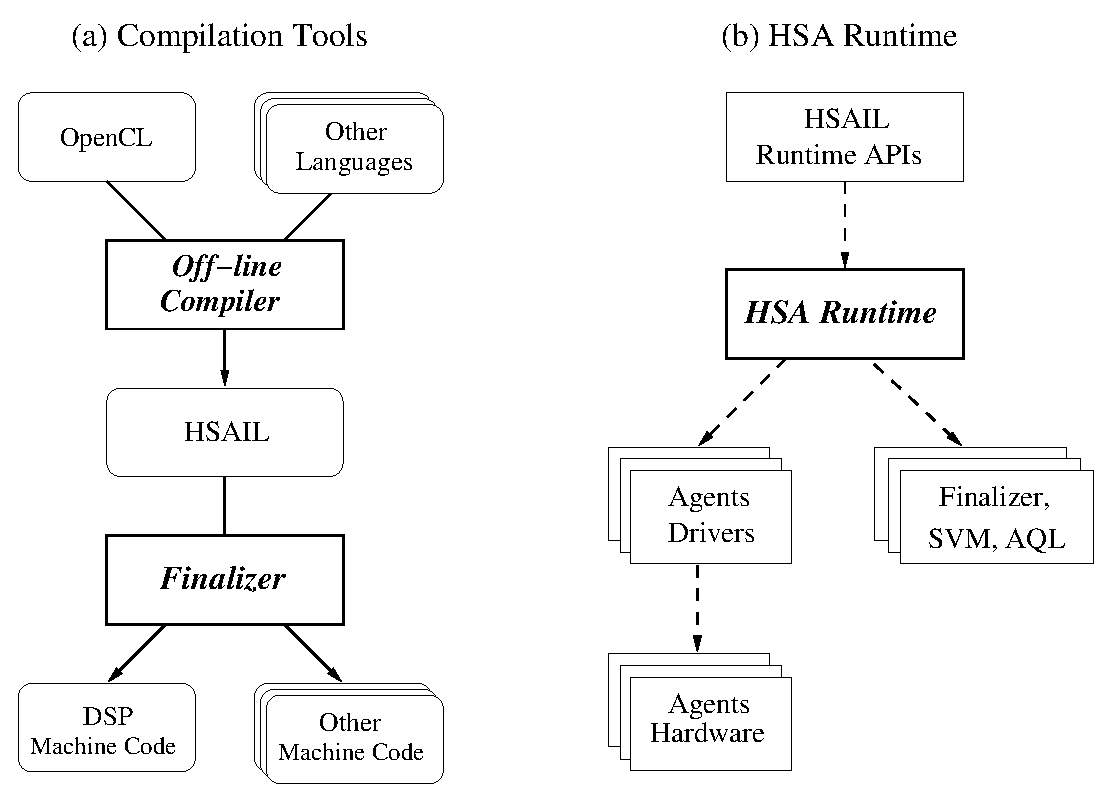
\includegraphics[width=0.8\textwidth]{./figs/swinf.eps}
            %        \label{fig:swinf}
            %    \end{figure}
            %\end{frame}


            \section{Design and Implementation}

            \subsection{Hardware Design and Implementation}
            \begin{frame}{Basic Design Considerations}
                Considering a datapath with one adder, multiplier and shifter, We want... \\
                \begin{itemize}
                    \item \textbf{Multi-issue} capability of VLIW but \textbf{low cost} in RF
                        \begin{itemize}
                            \item Partition RF to \textbf{multi-bank}
                            \item Specialize purpose of each bank --- \textbf{load, store or intermediate bank}
                        \end{itemize}
                    \item \textbf{Forwarding} mechanism of ASIP but \textbf{flexibility}
                        \begin{itemize}
                            \item Buffer FU result with dedicated latch
                            \item \textbf{Program data transportation} from latch to FU
                        \end{itemize}
                    \item Simpler compiler design for banked RF
                        \begin{itemize}
                            \item Use one load, store and intermediate bank per instruction stream 
                            \item Let instruction streams work independently --- \textbf{simultaneous multi-threading} (SMT)
                        \end{itemize}
                    \item Best trading-off for SMT width --- \textbf{dual-thread}
                \end{itemize}
                \large{That's \textbf{D}ual-thr\textbf{e}ad \textbf{Ar}chitecture}
            \end{frame}

            \begin{frame}{DeAr Micro-architecture}
                \begin{columns}
                    \begin{column}{0.6\textwidth}
                        \begin{figure}[!ht] 
                            \centering
                            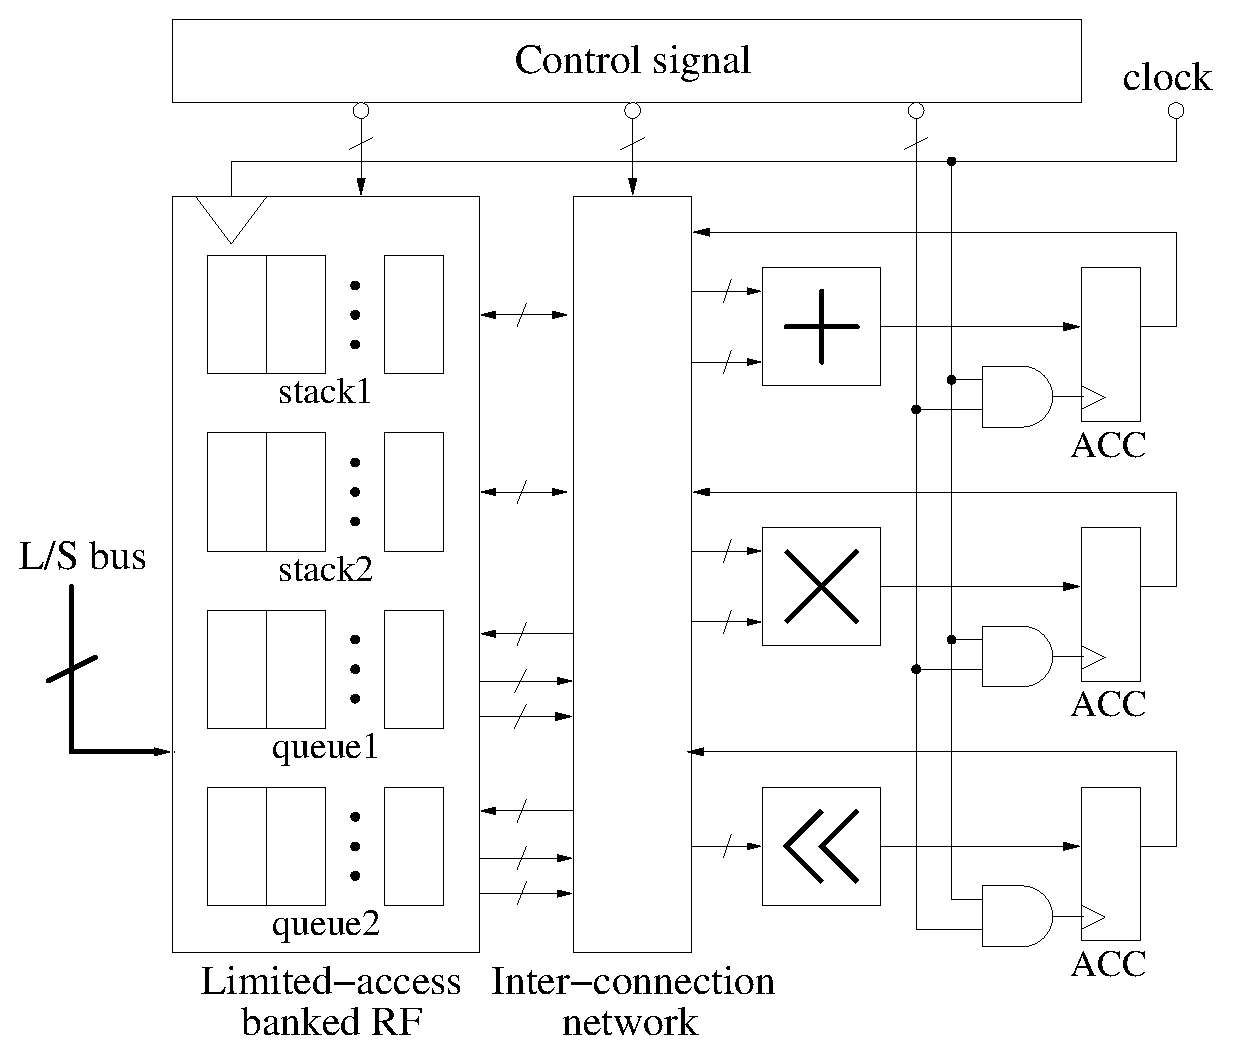
\includegraphics[width=1.0\textwidth]{./figs/micro.eps}
                        \end{figure}
                    \end{column}
                    \begin{column}{0.35\textwidth}
                        \begin{block}<2->{Key components}
                            \begin{itemize}
                                \item <3->
                                {
                                    \begin{itemize}
                                        \item Two load-banks
                                        \item Two store-banks
                                        \item Two intermediate-banks
                                    \end{itemize}
                                }
                                \item <4->{Transport Triggered Data Bus}
                                \item <5->{Accumulator latches}
                            \end{itemize}    
                        \end{block}
                    \end{column}
                \end{columns}
            \end{frame}

            \begin{frame}{Advanced Design Considerations}
                \begin{itemize}
                    \item Data flow is often binary tree like and used exactly once (vector, matrix, convolution, etc)
                        \begin{itemize}
                            \item Load data in use-order $\implies$ load bank is first-in first-out (FIFO)
                            \item Store data in WB-order $\implies$ store bank is first-in first-out (FIFO)
                            \item Post-order process binary tree $\implies$ intermediate bank is last-in first-out (LIFO)
                        \end{itemize}
                    \item Replacing random-access memory with queues and stacks
                        \begin{itemize}
                            \item Fewer bits to access RF $\implies$ better code density, lower decode complexity
                            \item Sequential load/store (L/S) $\implies$ burst memory transfer
                        \end{itemize}
                \end{itemize}
                \animategraphics[loop,controls,width=\linewidth]{12}{./figs/tree.gif}{0}{16}

            \end{frame}

            %\begin{frame}{Micro-architecture (2/2)}
            %    \begin{itemize}
            %        \item <2->{Sequential-access Banked RF (SBRF)
            %                \begin{itemize}
            %                    \item <3->{Load/store queues buffer memory transfer data}
            %                    \item <4->{Stack memory stores intermediate data}
            %                    \item <5->{Physical and symmetric separation for threads}
            %                    \item <6->{Implicit access reducing code size}
            %                \end{itemize}
            %            }
            %        \item <7->{Accumulator latches (ACCs) \\ --- buffering arithmetic results for future reuse}
            %        \item <8->{Transport-triggered Data Bus (TTDB)
            %                \begin{itemize}
            %                    \item Flexible data transport between ACCs and FUs
            %                    \item Facilitating exhaustive data reuse
            %                \end{itemize}
            %            }
            %    \end{itemize}
            %\end{frame}

            \begin{frame}{Instruction Set Architecture (1/2)}
                Each DeAr instruction is composed of two portions:
                \begin{itemize}
                    \item <2->{Stack control portion: manipulating the stack memory}
                    \item <3->{RISC-fashion portion: a subset of common RISC ISA}
                \end{itemize}
                \begin{table}[ht!]
                    \centering
                    \caption{Stack access portion of a DeAr instruction}
                    \resizebox{0.9\textwidth}{!}
                    {
                        \begin{tabular}{|l|l|l|}
                            \hline
                            \multicolumn{1}{|c|}{\textbf{Name}} & \multicolumn{1}{c|}{\textbf{Meaning}} & \multicolumn{1}{c|}{\textbf{Note}} \\ \hline
                        PUSH & \begin{tabular}[c]{@{}l@{}}1. Add the head address by 1\\ 2. Write the new data to the head address\end{tabular} & \multirow{2}{*}{ \parbox{5cm}{A "pop" followed by a "push" is equivalent to a "modify"} } \\ \cline{1-2}
                        POP                               & \begin{tabular}[c]{@{}l@{}}1. Subtract the head address by 1\\ 2. Invalidate the previous head data\end{tabular} & \\ \hline
                            MODIFY                            & Modify the head data to to the new data & The head address remains \\ \hline
                            STALL                               & No operation & The head address and data remain \\ \hline
                        \end{tabular}
                    }
                \end{table}
            \end{frame}


            \begin{frame}{Instruction Set Architecture (2/2)}
                \begin{table}[ht!]
                    \centering
                    \caption{RISC-fashion portion of a DeAr instruction}
                    \resizebox{0.8\textwidth}{!}
                    {
                        \begin{tabular}{|c|l|l|c|}
                            \hline
                            \multicolumn{1}{|c|}{\textbf{Category}} & \multicolumn{1}{c|}{\textbf{Name}} & \multicolumn{1}{c|}{\textbf{Meaning}} & \multicolumn{1}{c|}{\textbf{Target}} \\ \hline
                        \multirow{7}{*}{ \begin{tabular}[c]{@{}l@{}} \\ A type \end{tabular}}      & ADD & \textbf{d} = \textbf{s} + \textbf{t}  & \multirow{7}{*}{\begin{tabular}[c]{@{}l@{}} \\ Datapath \end{tabular}}  \\ \cline{2-3}
                                                                                                   & SUB & \textbf{d} = \textbf{s} $-$ \textbf{t} & \\ \cline{2-3} 
                                                                                                   & MUL & \textbf{d} = \textbf{s} $\times$ \textbf{t} & \\ \cline{2-3} 
                                                                                                   & SHL & \textbf{d} = \textbf{s} $<<$ \textbf{t} & \\ \cline{2-3}
                                                                                                   & SHR & \textbf{d} = \textbf{s} $>>$ \textbf{t} & \\ \cline{2-3}
                                                                                                   & MV  & \textbf{d} = \textbf{s} + 0 or \textbf{d} = \textbf{s} << 0 & \\ \cline{2-3} 
                                                                                                   & NOP & \begin{tabular}[c]{@{}l@{}}1. disable write back \\ 2. clock-gate the accumulator \end{tabular}& \\ \hline
                        \multirow{3}{*}{ \begin{tabular}[c]{@{}l@{}} \\ \\ B type \end{tabular}}          & JMP & pc = pc + \textbf{a}  & \multirow{3}{*}{ \begin{tabular}[c]{@{}l@{}} \\ \\ Instruction unit \end{tabular}} \\ \cline{2-3}
                                                                                                          & BZ  & \begin{tabular}[c]{@{}l@{}} \textit{if}(stack1.read() == stack2.read())\\ \ \ \ \ \ \ \ pc = pc + \textbf{a} \end{tabular} & \\ \cline{2-3}
                                                                                                          & BNZ & \begin{tabular}[c]{@{}l@{}} \textit{if}(stack1.read() != stack2.read())\\ \ \ \ \ \ \ \ pc = pc + \textbf{a} \end{tabular} & \\ \hline
                        \multirow{2}{*}{ \begin{tabular}[c]{@{}l@{}} \\ M type \end{tabular}}           & LD  & \begin{tabular}[c]{@{}l@{}} \textit{repeat}(\textbf{r})\\ \ \ \ \ \ \ \ load\_queue.push (memory[\textbf{a}]) \end{tabular}& \multirow{2}{*}{\begin{tabular}[c]{@{}l@{}} \\  Load/store unit \end{tabular}} \\ \cline{2-3} 
                                                                                                        & ST  & \begin{tabular}[c]{@{}l@{}} \textit{repeat}(\textbf{r})\\ \ \ \ \ \ \ \ memory[\textbf{a}] = store\_queue.pop() \end{tabular}& \\ \hline
                        \end{tabular}
                    }
                \end{table}
            \end{frame}

            \begin{frame}{Integrating DeAr with HSA (1/3)}
                \begin{columns}
                    \begin{column}{0.6\textwidth}
                        \begin{figure}[!ht] 
                            \centering
                            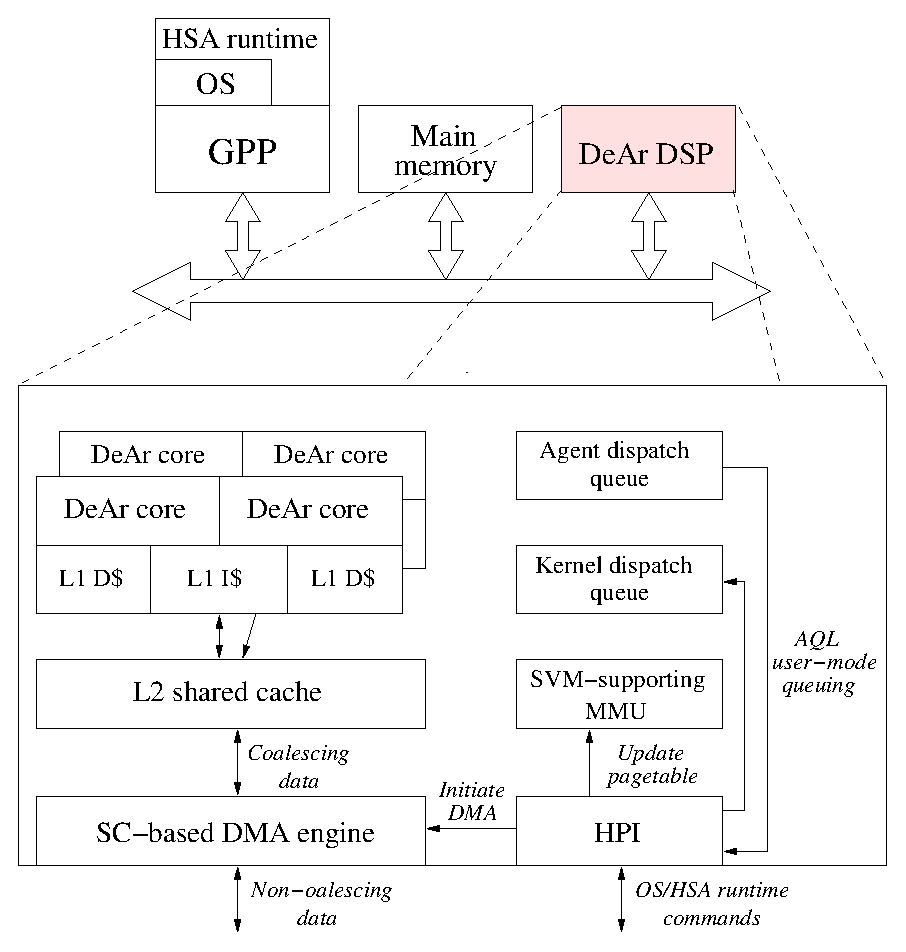
\includegraphics[width=1.0\textwidth]{./figs/archi.eps}
                            \label{fig:archi}
                        \end{figure}
                    \end{column}
                    \begin{column}{0.40\textwidth}
                        \begin{block}<2->{Key components}
                            \begin{itemize}
                                \item <3->{Multi-core DeAr with shared L1 I-cache}
                                \item <4->{Host port interface}
                                \item <5->{SC-based direct memory access engine}
                            \end{itemize}
                        \end{block}
                    \end{column}
                \end{columns}
            \end{frame}

            \begin{frame}{Integrating DeAr with HSA (2/3)}
                \begin{itemize}
                    \item <2-> {Multi-core DeAr with shared L1 I-cache~\cite{kelly2004shared} --- fitting HSA SPMD programming model and eliminating program data duplication}
                    \item <3-> {Host port interface (HPI)~\cite{hpi}
                            \begin{itemize}
                                \item Enabling host direct access to DeAr
                                \item Offloading MMU, AQL and SC control overhead to host
                            \end{itemize}
                        }
                    \item <4-> {SC-based DMA engine~\cite{sc}
                            \begin{itemize}
                                \item Performing data transfer and converting data layout on-the-fly
                                \item Improving data locality for DeAr by coalescing access pattern
                                \item Multiple Load/Store (L/S) instructions can be merged into one
                            \end{itemize}
                        }
                \end{itemize}
            \end{frame}

            \begin{frame}{Integrating DeAr with HSA (3/3)}
                \begin{itemize}
                    \item <2-> {Conventional architectures: referring to a work-item as a thread}
                    \item <3-> {DeAr: offloading a work-item to two DeAr threads\\ --- \textbf{FINER PARALLELISM}}
                \end{itemize}
                \begin{figure}[!ht]
                    \begin{center}
                        \setcounter{subfigure}{0}
                        \subfigure[Execution flow of an HSA work-item]
                        {
                            \label{fig:bb:1}
                            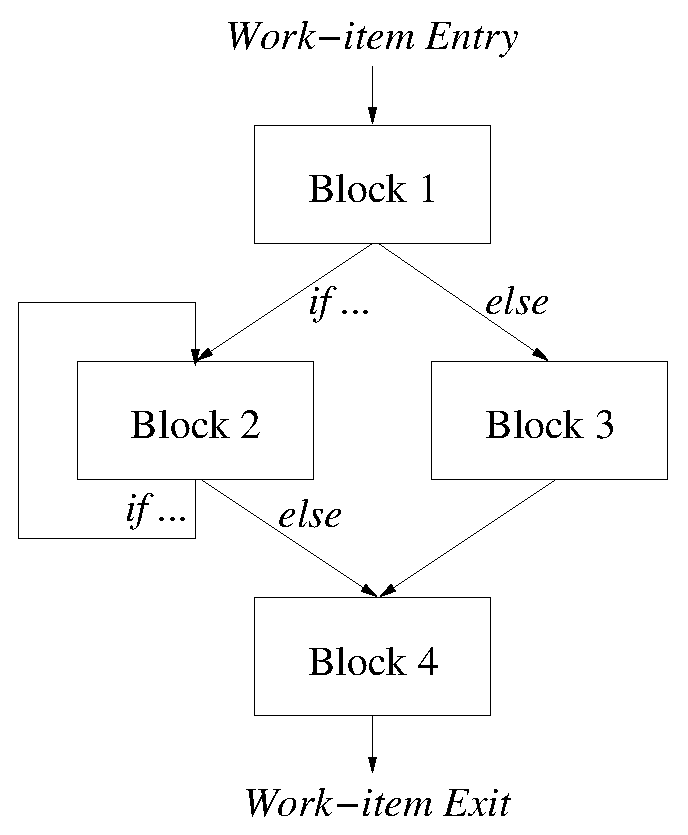
\includegraphics[width=0.33\textwidth]{figs/bb.eps}
                        }
                        \hfill
                        \subfigure[Accelerating the execution of a Basic block]
                        {
                            \label{fig:bb:2}
                            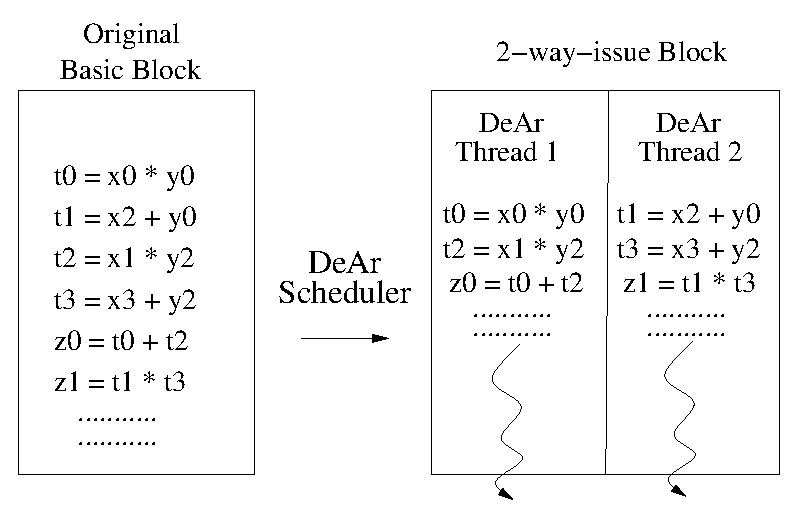
\includegraphics[width=0.55\textwidth]{figs/bb2.eps}
                        }
                    \end{center}
                \end{figure}
            \end{frame}

            \subsection{Software Design and Implementation}
            \begin{frame}{Software Framework}
                \begin{enumerate}
                    \item <2->{Compilation (front-end)
                            \begin{itemize}
                                \item DeAr users program in high level languages (OpenCL or C++)
                                \item Off-line compiler~\cite{cloc} from HSA foundation compiles them to HSAIL
                            \end{itemize}
                        }
                    \item <3->{Finalization (front-end)
                            \begin{itemize}
                                \item Converting HSAIL to data flow graph (DFG)
                                    \begin{itemize}
                                        \item Reaching definition analysis (RDA)
                                        \item Single static assignment (SSA)
                                    \end{itemize}
                                \item Converting DFG to hierarchical data flow graph (HDFG)
                            \end{itemize}
                        }
                    \item <4->{HDFG-based scheduling (back-end)
                            \begin{itemize}
                                \item OPC optimization --- inter-tree and intra-tree parallelism
                                \item Power optimization --- exhaustive forwarding
                                \item Memory footprint optimization --- LIFO fashion and minimum stack consumption
                                \item Code generation
                            \end{itemize}
                        }
                \end{enumerate}
            \end{frame}


            \begin{frame}{Finalization: Converting HSAIL to DFG}
                % \begin{algorithm}[H] \fontsize{10pt}{10pt}\selectfont  
                \begin{columns}
                    \begin{column}{0.45\textwidth}
                        \begin{block}{HSAIL: sum of products}
                            ld\_global\_u32 \$s2, [\$d0]; \\ 
                            ld\_global\_u32 \$s3, [\$d1]; \\ 
                            ld\_global\_u32 \$s2, [\$d2]; \\
                            ld\_global\_u32 \$s3, [\$d3]; \\
                            mul\_u32 \$s1, \$s2, \$s3; \\
                            mul\_u32 \$s4, \$s5, \$s6; \\
                            add\_u32 \$s7, \$s1, \$s4; \\
                            st\_global\_u32 \$s7, [\$d4]; \\
                        \end{block} 
                    \end{column}
                    \begin{column}{0.55\textwidth}
                        \begin{enumerate}
                            \item <2->{RDA retrieves use-define chains.}
                            \item <3->{SSA renames variables.
                                \begin{itemize}
                                    \item Give a new name to each LHS variable
                                    \item Update corresponding RHS based on RDA
                                \end{itemize}
                            }
                        \item <4->{Re-traversing new code
                                \begin{itemize}
                                    \item Store assignments in $V_{OP}$
                                    \item Store dependencies in $E_{OP}$
                                \end{itemize}
                            }
                        \item <5->{DFG: $G = (V_{OP}, E_{OP})$ is obtained.
                                \begin{itemize}
                                    \item Vertex: operation
                                    \item Edge: data flow
                                \end{itemize}
                            }
                        \end{enumerate}
                    \end{column}
                \end{columns}
            \end{frame}

            \begin{frame}{Finalization: Converting DFG to HDFG}
                \begin{itemize}
                    \item <2->{Conventional DSP program analysis: data flow graph (DFG) analysis}
                    \item <3->{We propose \textbf{Hierarchical data flow graph (HDFG)} \\
                            %--- providing abundant information for optimizations
                        }
                    \item <4->{After conversion, HDFG: $\bar{G} = (V_{BT}, E_{BT})$ is obtained. \\
                            --- \textbf{vertex}: binary tree $BT$, \textbf{edge}: data flow cross $BT$
                        }
                \end{itemize}
                \setcounter{subfigure}{0}
                \begin{figure}[!ht]
                    \begin{center}
                        \subfigure[DFG example]
                        {
                            \label{fig:dfg:dfg}
                            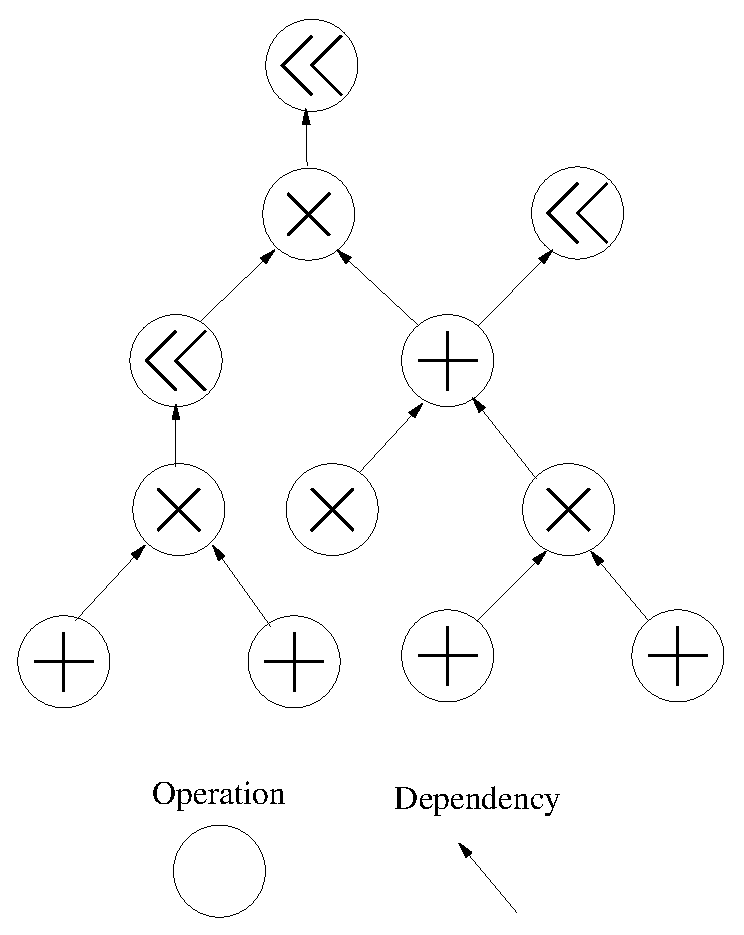
\includegraphics[width=0.32\textwidth]{figs/dfg.eps}
                        }
                        \subfigure[Corresponding HDFG]
                        {
                            \label{fig:dfg:hdfg}
                            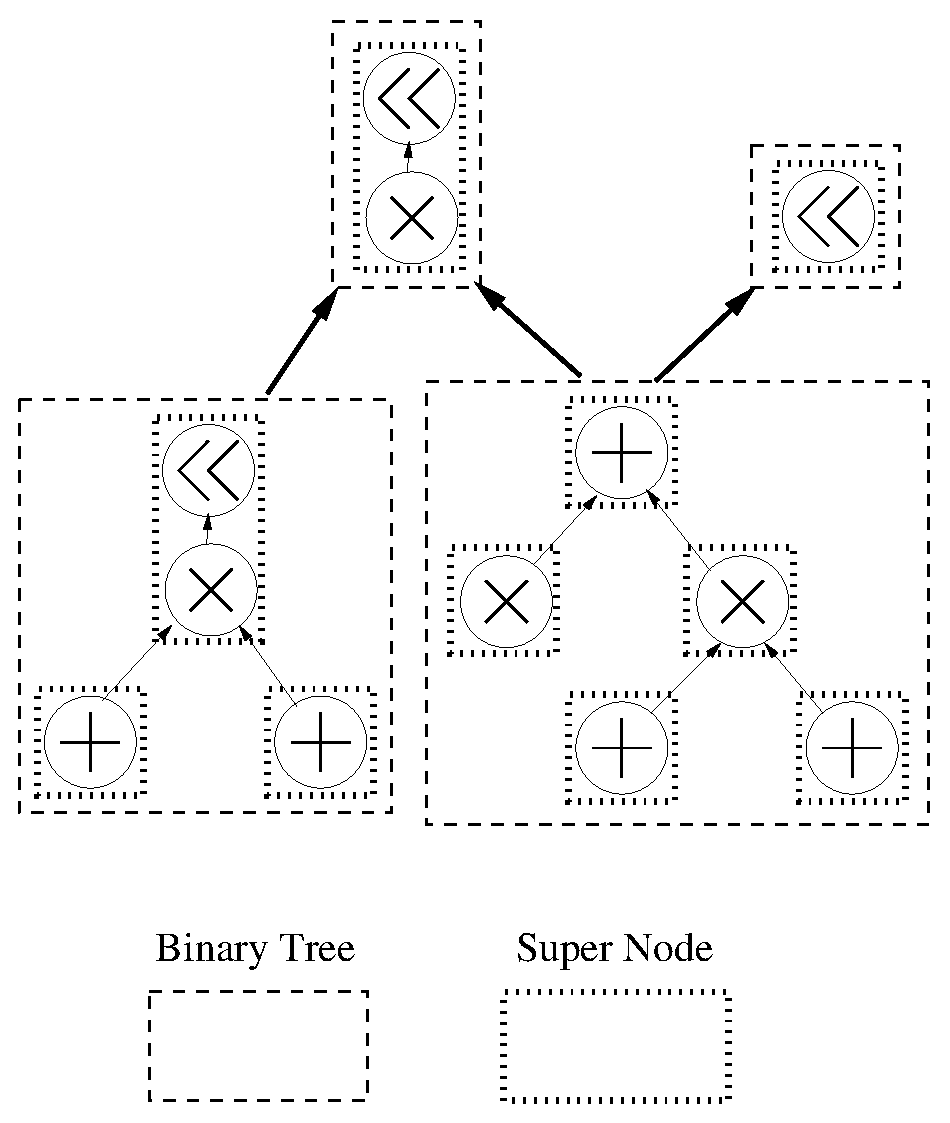
\includegraphics[width=0.32\textwidth]{figs/hdfg.eps}
                        }
                    \end{center}
                \end{figure}
            \end{frame}

            %\begin{frame}{Compilation: Properties of HDFG}
            %    \begin{itemize}
            %        \item <2->{Cascaded or isolated $OP$ form $SN$ \\ --- data forwarding must performed within $sn$.}
            %        \item <3->{Neighboring or isolated $SN$ form full binary tree $BT$ \\
            %                --- parent $SN$ receives data from stack and TTDB
            %                \begin{itemize}
            %                    \item First operand popped from stack
            %                    \item Second operand forwarded from TTDB
            %                \end{itemize}
            %            }
            %        \item <4->{Within a $BT$, a parent $SN$ receives the first operand popped from the stack and the second one forwarded via TTDB.}
            %        \item <5->{Dependencies among $SN$ that cross $BT$ are inherited}
            %        \item <6->{After scheduled, $BT$ and its edges are erased from HDFG}
            %    \end{itemize}
            %\end{frame}



            \begin{frame}{HDFG-based scheduling: Inter-tree parallelism}
                \only <2->{\textbf{Achieving high OPC by exploring parallelism in HDFG}}
                \begin{itemize}
                    \item <3->{A $BT$ without in-edges is free to be scheduled to a thread
                        \begin{itemize}
                            \item Operations in $BT$ are turned into a list
                            \item The thread executes operations on the list one by one
                        \end{itemize}
                    }
                \item <4->{Two free $BT$s are \textbf{parallelizable} --- \textbf{inter-tree parallelism}
                        \begin{itemize}
                            \item Processed by two threads respectively and concurrently.
                            \item Proceeding until all $BT$ are consumed
                        \end{itemize}
                    }
                \end{itemize}
                \only <5->{But sometimes...}
                \begin{itemize}
                    \item <6->{Only one $BT$ exists in HDFG at beginning}
                    \item <7->{One $BT$ remains after scheduling}
                    \item <8->{One partial $BT$ remains after scheduling}
                \end{itemize}
                \vspace{1em}
                \centering
                \only<9->{\textbf{Exploring intra-tree parallelism!}}
            \end{frame}

            \begin{frame}{HDFG-based scheduling: Intra-tree parallelism}
                \begin{columns}
                    \begin{column}{0.35\textwidth}
                    \end{column}
                    \begin{column}{0.65\textwidth}
                        \begin{itemize}
                            \item <2->{Partitioning $bt$ into three parts --- root, left and right-subtrees
                                \begin{itemize}
                                    \item Root: can only be handled sequentially
                                    \item Left and right-subtrees --- \textbf{intra-tree parallelism}, processed by two threads concurrently
                                \end{itemize}
                            }
                        \item <3->{Imbalance subtree size lead to smaller $bt$ remaining after scheduling}
                        \item <4->{Recursively partitioning and scheduling until completion}
                        \end{itemize} 
                        \vspace{1em} 
                        \only<5->{Parallelism is good, but how to handle \textbf{ALU conflict}?\\}
                        \vspace{1em} 
                        \centering
                        \only<6->{\textbf{DP-based ALU-allocation!}}
                    \end{column}
                \end{columns}
            \end{frame}

            \begin{frame}{HDFG-based scheduling: DP-based ALU-Allocation}
                    \setcounter{subfigure}{0}
                    \begin{figure}[!ht]
                        \begin{center}
                            \subfigure[Stage 1: scoring table modeling]
                            {
                                \label{fig:alloc:1}
                                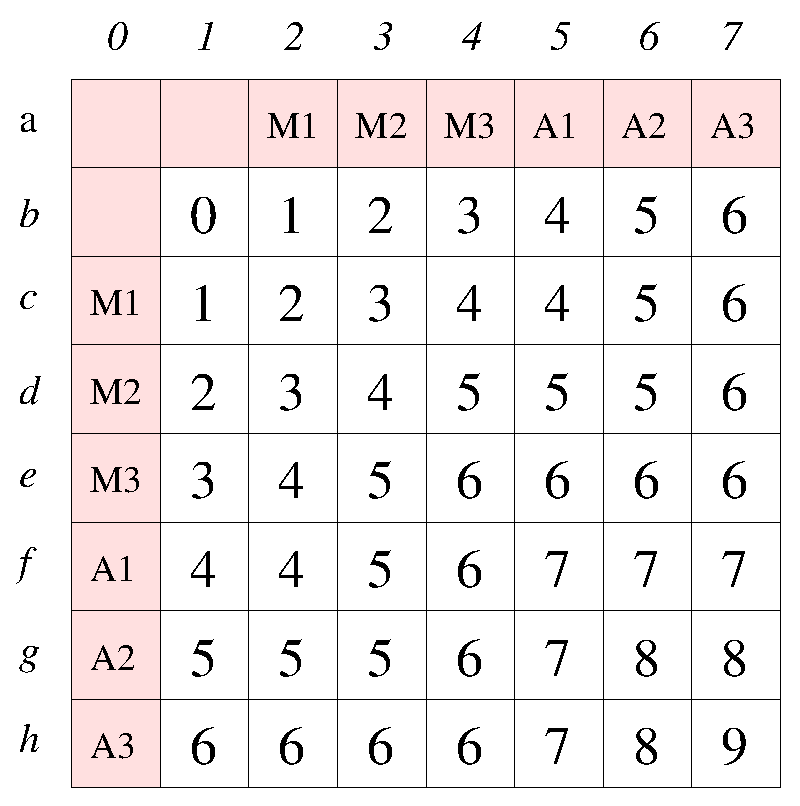
\includegraphics[width=0.3\textwidth]{figs/alloc.eps}
                            }
                            \hfill
                            \subfigure[Stage 2: scoring table filling]
                            {
                                \label{fig:alloc:2}
                                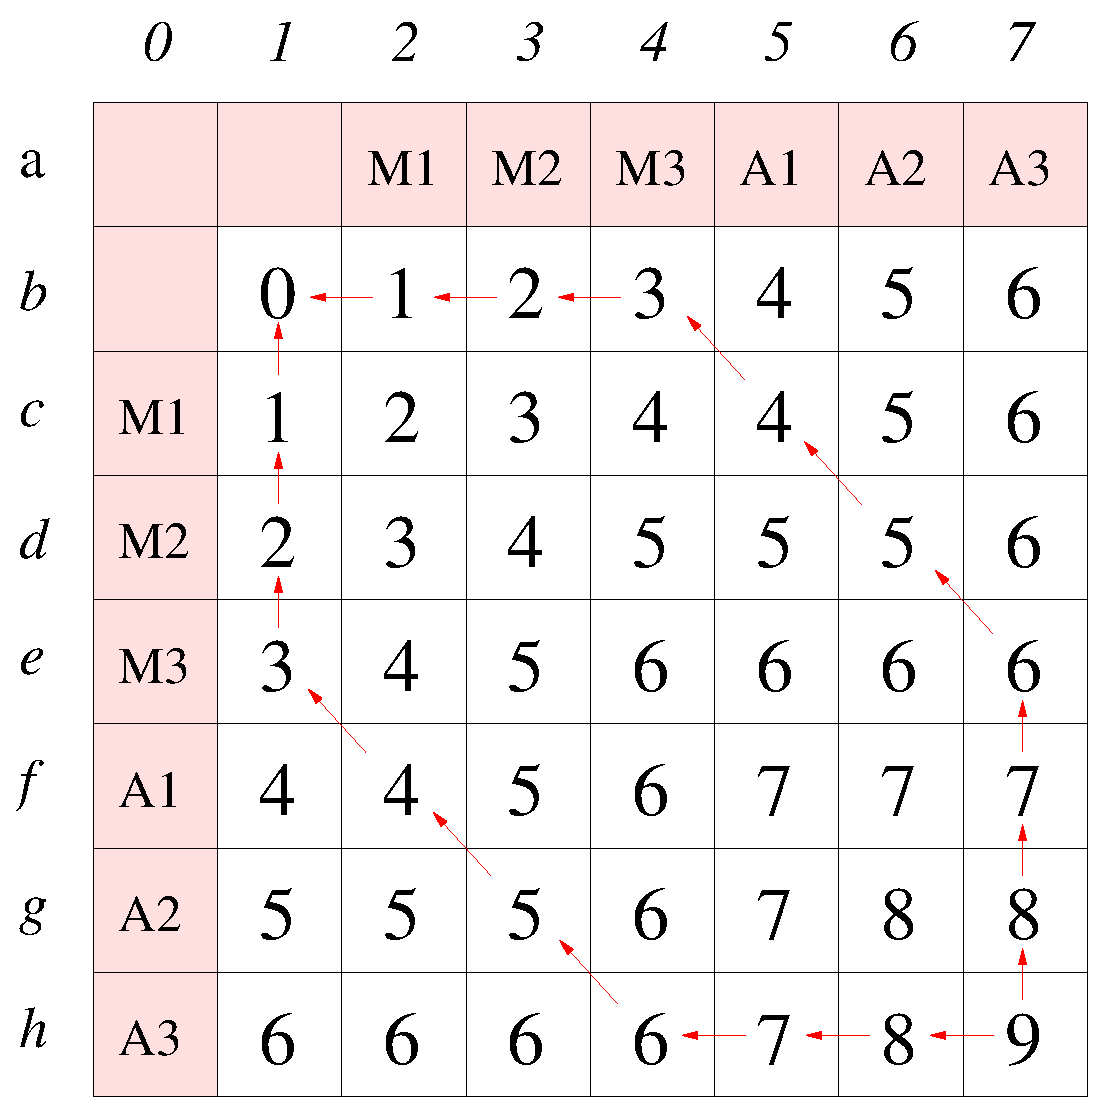
\includegraphics[width=0.3\textwidth]{figs/alloc2.eps}
                            }
                            \hfill
                            \subfigure[Stage 3: backtracking]
                            {
                                \label{fig:alloc:3}
                                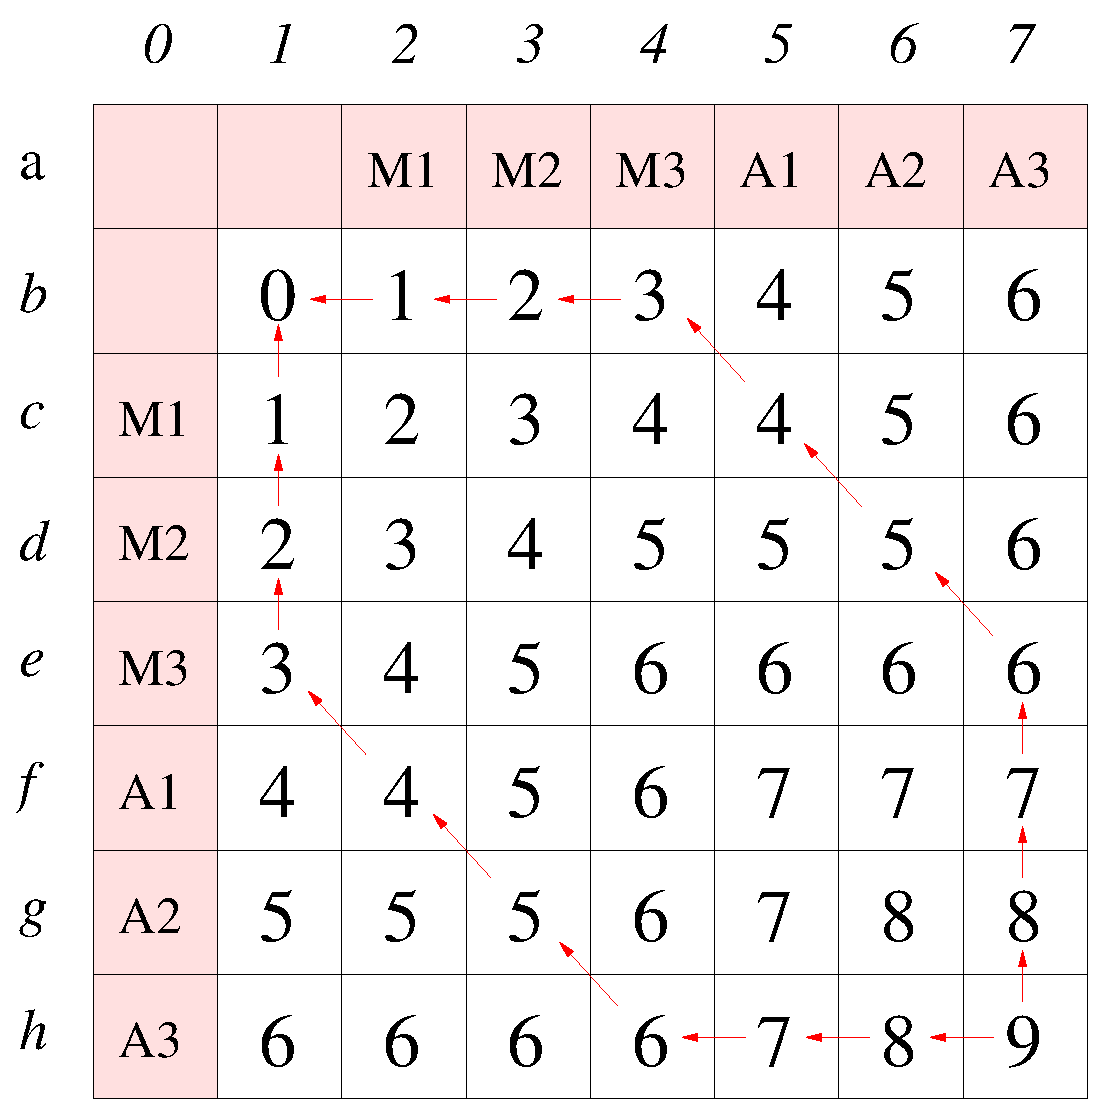
\includegraphics[width=0.3\textwidth]{figs/alloc3.eps}
                            }
                        \end{center}
                        \label{fig:alloc}
                    \end{figure}
                \begin{itemize}
                    \item <2-> {Analyzing operation-lists of two threads by Dynamic programming (DP) and performing ALU-allocation}
                    \item <3-> {DP determines which thread stalls at conflict, achieving optimal OPC}
                    \item <4-> {An example where two threads have MMMAAA in their operation-lists}
                \end{itemize}
            \end{frame}

            %\begin{frame}{HDFG-based scheduling: HFPT sort}
            %    \begin{figure}[!h]
            %        \begin{center}
            %            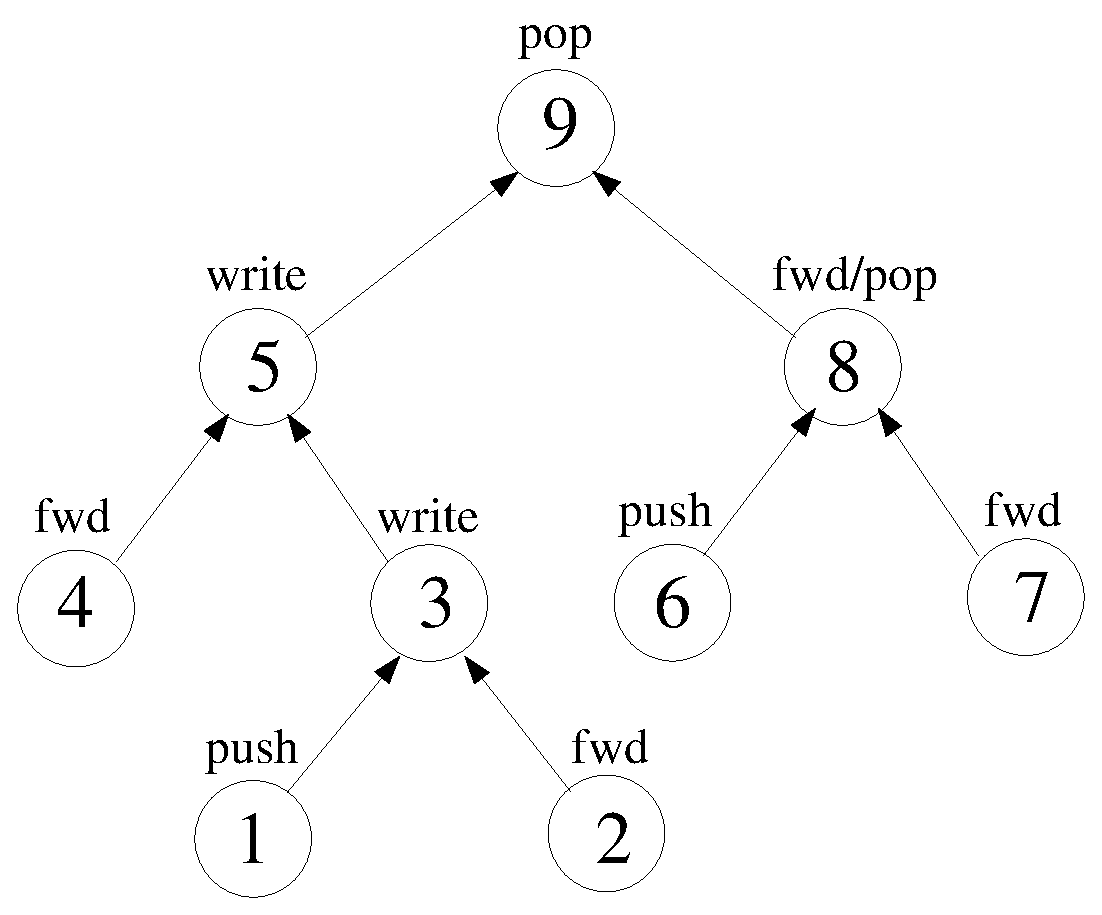
\includegraphics[width=0.4\textwidth]{figs/hfpt.eps}
            %        \end{center}
            %        \label{fig:hfpt}
            %    \end{figure}%
            %    \begin{itemize}
            %        \item <2->{HFPT (higher-first post-order) sort determines exeuction order in $BT$}
            %        \item <3->{Post-order traversal ensures LIFO memory footprint \\ --- \textbf{achieving flexibility}}
            %        \item <4->{Higher-first strategy lets higher subtree go first \\ --- \textbf{minimizing stack consumption}}
            %        \item <5->{$OP$s in $SN$ are atomic where data must flows via forwarding bus \\ -- \textbf{reducing power}}
            %    \end{itemize}
            %\end{frame}



            \section{Performance Evaluation}
            \subsection{Experiment Setup}
            %\begin{frame}{Why Single-core Evaluation?}
            %    \begin{itemize}
            %        \item <2->{Multi-core performance is highly correlated with issues not discussed in this work.
            %                \begin{itemize}
            %                    \item Core interconnection
            %                    \item Memory subsystem 
            %                    \item Shared memory or message passing
            %                \end{itemize}
            %            }
            %        \item <3->{Programming language also plays a crucial role, but popular ones are still contending for becoming the standard. \\
            %            --- HSA, OpenCL, CUDA, OpenMP, etc.
            %        }
            %        \item <4->{Benchmarking multi-core DSP is still an open field of study~\cite{landscape}}
            %    \end{itemize}       
            %\end{frame}
            \begin{frame}{Simulation Benchmark Suites}
                \begin{table}[!ht]
                    \centering
                    \resizebox{\columnwidth}{!}
                    {
                        \begin{tabular}{|c|c|c|c|c|c|c|c|c|}
                            \hline
                            \multicolumn{9}{|c|}{\textbf{Basic linear algebra subprograms (BLAS)}} \\ \hline
                            Benchmark              & AXPY   & MV     & MM      & INV      & CAXPY  & CMV  & CMM    & CINV  \\ \hline
                            \# add            &  32    &  56    &   48    &    75    &  128   & 132  &   90   &  88   \\ \hline
                            \# mul            &  32    &  64    &   64    &   172    &  128   & 144  &  108   & 114   \\ \hline
                            \# sht            &   0    &   0    &    0    &     0    &    0   &   0  &    0   &   0   \\ \hline
                            \# op             &  64    & 120    &  112    &   247    &  256   & 276  &  198   & 202   \\ \hline
                            \multicolumn{9}{|c|}{\textbf{General DSP kernels (GDSPK)}}                     \\ \hline
                            Benchmark              & FIR    & CFIR   & LPFIR   & Biquad   & IT     & DCT  & IMDCT  & FFT   \\ \hline
                            \# add            & 15     &  62    &   15    &    8     &  32    &  29  &   21   &  23   \\ \hline
                            \# mul            & 16     &  64    &    8    &    9     &   0    &  12  &   11   &  10   \\ \hline
                            \# sht            &  0     &   0    &    0    &    0     &  10    &   9  &    9   &   0   \\ \hline
                            \# op             & 31     & 126    &   23    &   17     &  42    &  50  &   41   &  33   \\ \hline
                        \end{tabular}
                    }
                \end{table}
                \begin{itemize}
                    \item Three primitive operations --- addition, multiplication and shifting.
                    \item BLAS --- classic matrix/vector library for wireless communication.
                    \item GDSPK --- common DSP filters and transformation algorithms.
                \end{itemize}
            \end{frame}

            \begin{frame}{Simulation Environment}
                \begin{figure}[!ht] 
                    \centering
                    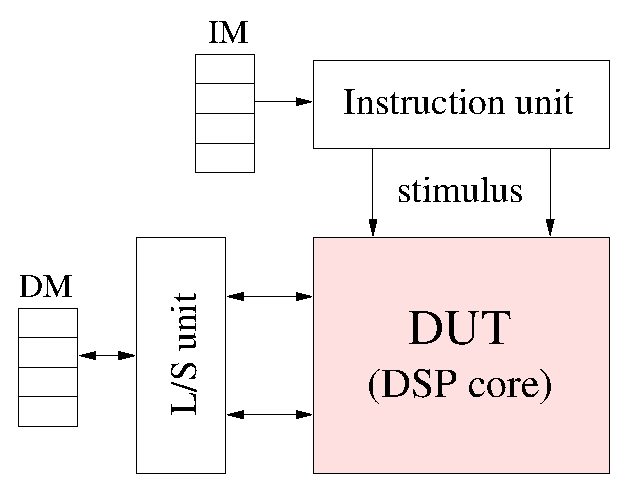
\includegraphics[width=0.45\textwidth]{./figs/sim.eps}
                \end{figure}
                \begin{itemize}
                    \item <2->{DUT is replaced with \textbf{DeAr}, \textbf{scalar}, \textbf{VLIW} and \textbf{composite-ALU} (cascade-ALU ASIP) in accordance.}
                    \item <3->{Composite-ALU is evaluated with best two ALU configurations (MSA and AMS) respectively.}
                    \item <4->{Designs have compatible RF (32 cells) and ALU resources (one adder, multiplier and shifter).}
                \end{itemize}
            \end{frame}

            \subsection{Pre-synthesis Analysis}

            \begin{frame}{Operations per Cycle}
                \begin{table}[!ht]
                    \centering
                    \resizebox{\columnwidth}{!}
                    {
                        \begin{tabular}{|c|c|c|c|c|c|c|c|c|c|}
                            \hline
                            \multicolumn{10}{|c|}{\textbf{Basic linear algebra subprograms (BLAS)}} \\ \hline
                            Benchmark  &  AXPY  &  MV  &  MM  &  MINV  &  CAXPY  &  CMV  &  CMM  &  CMINV  &  Average \\ \hline 
                            VLIW  &   1.94  &   1.85  &   1.72  &   1.44  &   1.97  &   1.89  &   1.80  &   1.76  &   1.79     \\ \hline 
                            DeAr  &   1.94  &   1.85  &   1.72  &   1.40  &   1.97  &   1.89  &   1.80  &   1.62  &   1.77     \\ \hline
                            Composite-MSA  &   2.00  &   1.88  &   1.75  &   1.37  &   1.33  &   1.35  &   1.38  &   1.53  &   1.57     \\ \hline 
                            Composite-AMS  &   1.00  &   1.00  &   1.00  &   1.02  &   1.00  &   1.00  &   1.00  &   1.04  &   1.01     \\ \hline 
                            Scalar  & 1.0  & 1.0  & 1.0  & 1.0  & 1.0  & 1.0  & 1.0  & 1.0  & 1.0 \\ \hline 
                            \multicolumn{10}{|c|}{\textbf{General DSP application kernels (GDSPK)}}                     \\ \hline
                            Benchmark  &  FIR  &  CFIR  &  LPFIR  &  Biquad  &  IT  &  DCT  &  IMDCT  &  FFT  &  Average \\ \hline 
                            VLIW  &   1.82  &   1.91  &   1.67  &   1.55  &   1.33  &   1.61  &   1.86  &   1.38  &   1.64     \\ \hline 
                            DeAr  &   1.82  &   1.91  &   1.67  &   1.55  &   1.33  &   1.47  &   1.46  &   1.32  &   1.57     \\ \hline 
                            Composite-MSA  &   1.94  &   1.34  &   1.44  &   1.42  &   1.31  &   1.14  &   1.28  &   1.06  &   1.35     \\ \hline 
                            Composite-AMS  &   1.00  &   1.00  &   1.53  &   1.21  &   1.14  &   1.61  &   1.52  &   1.27  &   1.29     \\ \hline 
                            Scalar  & 1.0  & 1.0  & 1.0  & 1.0  & 1.0  & 1.0  & 1.0  & 1.0  & 1.0 \\ \hline 
                        \end{tabular}
                    }
                \end{table}
                \begin{itemize}
                    \item <2->{VLIW benefits from most flexible datapath so it achieves best OPC.}
                    \item <3->{Composite-ALU OPC is impacted by matchability between ALU order and benchmark characteristic.}
                    \item <4->{By leveraging HDFG-based scheduling, DeAr have only 1.11\% and 4.26\% loss against VLIW,
                        and remove redundant connection in RF.}
                \end{itemize}

            \end{frame}

            \begin{frame}{Register File Access Rate}
                \begin{table}[!ht]
                    \centering
                    \resizebox{\columnwidth}{!}
                    {
                        \begin{tabular}{|c|c|c|c|c|c|c|c|c|c|}
                            \hline
                            \multicolumn{10}{|c|}{\textbf{Basic linear algebra subprograms (BLAS)}} \\ \hline
                            Benchmark  &  AXPY  &  MV  &  MM  &  MINV  &  CAXPY  &  CMV  &  CMM  &  CMINV  &  Average \\ \hline 
                            DeAr  &   0.67  &   0.69  &   0.71  &   0.67  &   0.67  &   0.68  &   0.70  &   0.71  &   0.69     \\ \hline
                            Composite-MSA  &   0.67  &   0.69  &  0.71  &   0.82  &   0.83  &   0.83  &   0.82  &   0.77  &  0.77     \\ \hline 
                            Composite-AMS  &   1.0  &   1.00  &   1.00  &   0.98  &   1.00  &   1.00  &   1.00  &   0.97  &   0.99     \\ \hline 
                            VLIW  &   1.00  &   1.00  &   1.00  &   1.00  &   1.00  &   1.00  &   1.00  &   1.00  &   1.00     \\ \hline 
                            Saclar  &   1.00  &   1.00  &   1.00  &   1.00  &   1.00  &   1.00  &   1.00  &   1.00  &   1.00     \\ \hline 
                            \multicolumn{10}{|c|}{\textbf{General DSP kernels (GDSPK)}}                     \\ \hline
                            Benchmark  &  FIR  &  CFIR  &  LPFIR  &  Biquad  &  IT  &  DCT  &  IMDCT  &  FFT  &  Average \\ \hline 
                            DeAr  &   0.68  &   0.67  &  0.60  &   0.57  &   0.85  &   0.74  &   0.86  &   0.82  &   0.73     \\ \hline 
                            Composite-MSA  &   0.68  &   0.83  &   0.80  &   0.80  &   0.83  &   0.87  &   0.80  &   0.92  &   0.82     \\ \hline 
                            Composite-AMS  &   1.00  &   1.00  &   0.77  &   0.88  &   1.00  &   0.76  &   0.84  &   0.86  &   0.87     \\ \hline 
                            VLIW  &   1.00  &   1.00  &   1.00  &   1.00  &   1.00  &   1.00  &   1.00  &   1.00  &   1.00     \\ \hline 
                            Saclar  &   1.00  &   1.00  &   1.00  &   1.00  &   1.00  &   1.00  &   1.00  &   1.00  &   1.00     \\ \hline 
                        \end{tabular}
                    }
                \end{table}
                \begin{itemize}
                    \item <2->{Under assumption of single cycle, VLIW and scalar lack forwarding mechanism so have worst access rate.}
                    \item <3->{Composite-ALU forwarding capability is limited by the cascaded order and length.}
                    \item <4->{DeAr achieves lowest RF access rate by leveraging HDFG-based scheduling.}
                \end{itemize}
            \end{frame}

            \subsection{Synthesis Result and Analysis}

            \begin{frame}{Area}
                \setcounter{subfigure}{0}
                \begin{figure}[t]
                    \begin{center}
                        \subfigure[BLAS benchmark suite]
                        {
                            \label{chart:area:blas}
                            \includegraphics[width=0.48\textwidth]{charts/area_blas.eps}
                        }
                        \subfigure[General benchmark suite]
                        {
                            \label{chart:area:general}
                            \includegraphics[width=0.48\textwidth]{charts/area_general.eps}
                        }
                    \end{center}
                \end{figure}
                \begin{itemize}
                    \item <2->{DeAr outperforms either VLIW by 35.4\%--21.1\% and 35.2\%--21.6\%, 
                           ASIP by 21.2\%--5.3\% and 33.5\%--4.7\%, because of banked RF and lower decode complexity.}
                    \item <3->{Scalar suffers from low OPC and lead to dramatic growth while throughput is above 500 MOPS.}
                \end{itemize}
            \end{frame}

            \begin{frame}{Power Dissipation}
                \setcounter{subfigure}{0}
                \begin{figure}[t]
                    \begin{center}
                        \subfigure[BLAS benchmark suite]
                        {
                            \label{chart:power:blas}
                            \includegraphics[width=0.48\textwidth]{charts/power_blas.eps}
                        }
                        \subfigure[General benchmark suite]
                        {
                            \label{chart:power:general}
                            \includegraphics[width=0.48\textwidth]{charts/power_general.eps}
                        }
                    \end{center}
                \end{figure}
                \begin{itemize}
                    \item <2->{Linear growth regardless of design indicates the domination of dynamic power.}
                    \item <3->{DeAr outperforms either VLIW by 35.4\%--21.1\% and 35.2\%--21.6\%, 
                            or ASIP by 21.2\%--5.3\% and 33.5\%--4.7\%, because of lower area and RF access rate.}
                \end{itemize}
            \end{frame}

            \begin{frame}{Static Power Dissipation}
                \setcounter{subfigure}{0}
                \begin{figure}[t]
                    \begin{center}
                        \subfigure[BLAS benchmark suite]
                        {
                            \label{chart:leakage:blas}
                            \includegraphics[width=0.48\textwidth]{charts/leakage_blas.eps}
                        }
                        \subfigure[General benchmark suite]
                        {
                            \label{chart:leakage:general}
                            \includegraphics[width=0.48\textwidth]{charts/leakage_general.eps}
                        }
                    \end{center}
                \end{figure}
                \begin{itemize}
                    \item <2->{Very high correlation with area evaluation.}
                    \item <3->{DeAr outperforms either VLIW by 35.4\%--21.1\% and 35.2\%--21.6\%, or ASIP by 21.2\%--5.3\% and 33.5\%--4.7\%}
                \end{itemize}
            \end{frame}

            \section{Conclusion and Future Work}
            \begin{frame}{Conclusion Remarks}
                \begin{itemize}
                    \item <2->{Proposed DeAr DSP achieves power-efficient, flexibility and high OPC by leveraging the novel HDFG-based scheduling.}
                    \item <3->{Compared with VLIW and ASIP respectively, DeAr saves:
                            \begin{itemize}
                                \item 35.4\%--21.1\% and 21.2\%--5.3\% of area, 22.7\%--15.1\% and 46.9\%--2.8\% of power dissipation in BLAS.
                                \item 35.2\%--21.6\% and 33.5\%--4.7\% of area, 18.5\%--10.4\% and 19.7\%--1.5\% of power dissipation in GDSPK.
                            \end{itemize}
                        }
                    \item <4->{The compact design endows DeAr good scalability for multi-core architecture.}
                    \item <5->{To demonstrate the compatibility of DeAr with HSA standard, we present:
                            \begin{itemize}
                                \item The architecture framework of an HSA platform integrated with a multi-core DeAr.
                                \item The software framework of a HSA-compatible DeAr compiler.
                            \end{itemize}
                        }
                \end{itemize}
            \end{frame}

            \begin{frame}{Future Work}
                \begin{itemize}
                    \item <2->{Implementation of SC-based DMA engine~\cite{sc}
                            \begin{itemize}
                                \item Coalescing data layout and merging several L/S instructions into one.
                                \item Needing more studies for trading-off among throughput, power and flexibility. 
                            \end{itemize}
                        }
                    \item <3->{Using unused bits to enhance current DeAr ISA (interrupt, special function, etc.)}
                    \item <4->{Conducting system level emulation with HSAemu~\cite{hsaemu} to evaluate the memory hierarchy and multi-core design for DeAr.}
                    \item <5->{Exploring the possibilities of applying DeAr to GPU.
                            \begin{itemize}
                                \item Efficient DeAr core is a potential alternative to RISC shader
                                \item Dynamic massive threads management is the main challenge
                            \end{itemize}
                        }
                \end{itemize}

            \end{frame}

            \begin{frame}[plain,c]
                \centering
                \Huge{Thank You!}
            \end{frame}

            \begin{frame}[allowframebreaks]{Reference}
                \printbibliography
            \end{frame}


        \end{CJK}
        \end{document}


